\documentclass[11pt,compress,t,notes=noshow, xcolor=table]{beamer}
\usepackage[]{graphicx}\usepackage[]{color}
% maxwidth is the original width if it is less than linewidth
% otherwise use linewidth (to make sure the graphics do not exceed the margin)
\makeatletter
\def\maxwidth{ %
  \ifdim\Gin@nat@width>\linewidth
    \linewidth
  \else
    \Gin@nat@width
  \fi
}
\makeatother

\newcommand{\citebutton}[2]{%
\beamergotobutton{\href{#2}{#1}}%
}

\newcommand{\blu}[1]{\textcolor{blue}{#1}}
\newcommand{\org}[1]{\textcolor{orange}{#1}}
\newcommand{\ques}{\textbf{\textcolor{red}{Question:  }}}
\newcommand{\questionssofar}{\begin{frame}\frametitle{Any questions?}\end{frame}}

\newcommand\warning{%
 \makebox[1.4em][c]{%
 \makebox[0pt][c]{\raisebox{.1em}{\scriptsize!}}%
 \makebox[0pt][c]{\color{red}\normalsize$\bigtriangleup$}}}%

\definecolor{fgcolor}{rgb}{0.345, 0.345, 0.345}
\newcommand{\hlnum}[1]{\textcolor[rgb]{0.686,0.059,0.569}{#1}}%
\newcommand{\hlstr}[1]{\textcolor[rgb]{0.192,0.494,0.8}{#1}}%
\newcommand{\hlcom}[1]{\textcolor[rgb]{0.678,0.584,0.686}{\textit{#1}}}%
\newcommand{\hlopt}[1]{\textcolor[rgb]{0,0,0}{#1}}%
\newcommand{\hlstd}[1]{\textcolor[rgb]{0.345,0.345,0.345}{#1}}%
\newcommand{\hlkwa}[1]{\textcolor[rgb]{0.161,0.373,0.58}{\textbf{#1}}}%
\newcommand{\hlkwb}[1]{\textcolor[rgb]{0.69,0.353,0.396}{#1}}%
\newcommand{\hlkwc}[1]{\textcolor[rgb]{0.333,0.667,0.333}{#1}}%
\newcommand{\hlkwd}[1]{\textcolor[rgb]{0.737,0.353,0.396}{\textbf{#1}}}%
\let\hlipl\hlkwb

\usepackage{framed}
\makeatletter
\newenvironment{kframe}{%
 \def\at@end@of@kframe{}%
 \ifinner\ifhmode%
  \def\at@end@of@kframe{\end{minipage}}%
  \begin{minipage}{\columnwidth}%
 \fi\fi%
 \def\FrameCommand##1{\hskip\@totalleftmargin \hskip-\fboxsep
 \colorbox{shadecolor}{##1}\hskip-\fboxsep
     % There is no \\@totalrightmargin, so:
     \hskip-\linewidth \hskip-\@totalleftmargin \hskip\columnwidth}%
 \MakeFramed {\advance\hsize-\width
   \@totalleftmargin\z@ \linewidth\hsize
   \@setminipage}}%
 {\par\unskip\endMakeFramed%
 \at@end@of@kframe}
\makeatother

\definecolor{shadecolor}{rgb}{.97, .97, .97}
\definecolor{messagecolor}{rgb}{0, 0, 0}
\definecolor{warningcolor}{rgb}{1, 0, 1}
\definecolor{errorcolor}{rgb}{1, 0, 0}
\newenvironment{knitrout}{}{} % an empty environment to be redefined in TeX

\usepackage{alltt}
\newcommand{\SweaveOpts}[1]{}  % do not interfere with LaTeX
\newcommand{\SweaveInput}[1]{} % because they are not real TeX commands
\newcommand{\Sexpr}[1]{}       % will only be parsed by R
\newcommand{\xmark}{\ding{55}}%


\usepackage[english]{babel}
\usepackage[utf8]{inputenc}

\usepackage{dsfont}
\usepackage{verbatim}
\usepackage{amsmath}
\usepackage{amsfonts}
\usepackage{amssymb}
\usepackage{bm}
\usepackage{csquotes}
\usepackage{multirow}
\usepackage{longtable}
\usepackage{booktabs}
\usepackage{enumerate}
\usepackage[absolute,overlay]{textpos}
\usepackage{psfrag}
\usepackage{algorithm}
\usepackage{algpseudocode}
\usepackage{eqnarray}
\usepackage{arydshln}
\usepackage{tabularx}
\usepackage{placeins}
\usepackage{tikz}
\usepackage{setspace}
\usepackage{colortbl}
\usepackage{mathtools}
\usepackage{wrapfig}
\usepackage{bm}
\usepackage{amsmath}
\usepackage{pifont}

\usetikzlibrary{shapes.multipart,shapes,arrows,automata,positioning,calc,chains,trees, shadows}
\tikzset{
  %Define standard arrow tip
  >=stealth',
  %Define style for boxes
  punkt/.style={
    rectangle,
    rounded corners,
    draw=black, very thick,
    text width=6.5em,
    minimum height=2em,
    text centered},
  % Define arrow style
  pil/.style={
    ->,
    thick,
    shorten <=2pt,
    shorten >=2pt,}
}

\tikzstyle{vec}=[draw, rectangle, fill = white, minimum width=5mm, minimum height=1cm, inner sep = 2pt]

\usepackage{subfig}

% Defines macros and environments
\usepackage{../../style/lmu-lecture}


\let\code=\texttt
\let\proglang=\textsf

\setkeys{Gin}{width=0.9\textwidth}

\setbeamertemplate{frametitle}{\expandafter\uppercase\expandafter\insertframetitle}

\usepackage{bbm}
% basic latex stuff
\newcommand{\pkg}[1]{{\fontseries{b}\selectfont #1}} %fontstyle for R packages
\newcommand{\lz}{\vspace{0.5cm}} %vertical space
\newcommand{\dlz}{\vspace{1cm}} %double vertical space
\newcommand{\oneliner}[1] % Oneliner for important statements
{\begin{block}{}\begin{center}\begin{Large}#1\end{Large}\end{center}\end{block}}


%new environments
\newenvironment{vbframe}  %frame with breaks and verbatim
{
 \begin{frame}[containsverbatim,allowframebreaks]
}
{
\end{frame}
}

\newenvironment{vframe}  %frame with verbatim without breaks (to avoid numbering one slided frames)
{
 \begin{frame}[containsverbatim]
}
{
\end{frame}
}

\newenvironment{blocki}[1]   % itemize block
{
 \begin{block}{#1}\begin{itemize}
}
{
\end{itemize}\end{block}
}

\newenvironment{fragileframe}[2]{  %fragile frame with framebreaks
\begin{frame}[allowframebreaks, fragile, environment = fragileframe]
\frametitle{#1}
#2}
{\end{frame}}


\newcommand{\myframe}[2]{  %short for frame with framebreaks
\begin{frame}[allowframebreaks]
\frametitle{#1}
#2
\end{frame}}

\newcommand{\remark}[1]{
  \textbf{Remark:} #1
}


\newenvironment{deleteframe}
{
\begingroup
\usebackgroundtemplate{
\includegraphics[width=\paperwidth,height=\paperheight]{../style/color/red.png}}
 \begin{frame}
}
{
\end{frame}
\endgroup
}
\newenvironment{simplifyframe}
{
\begingroup
\usebackgroundtemplate{
\includegraphics[width=\paperwidth,height=\paperheight]{../style/color/yellow.png}}
 \begin{frame}
}
{
\end{frame}
\endgroup
}\newenvironment{draftframe}
{
\begingroup
\usebackgroundtemplate{
\includegraphics[width=\paperwidth,height=\paperheight]{../style/color/green.jpg}}
 \begin{frame}
}
{
\end{frame}
\endgroup
}
% https://tex.stackexchange.com/a/261480: textcolor that works in mathmode
\makeatletter
\renewcommand*{\@textcolor}[3]{%
  \protect\leavevmode
  \begingroup
    \color#1{#2}#3%
  \endgroup
}
\makeatother





\input{../../latex-math/basic-math.tex}
\input{../../latex-math/basic-ml.tex}
\usepackage{animate}

\newcommand{\titlefigure}{figure/metrics.png}
\newcommand{\learninggoals}{
\item Task-specific metrics
\item Metrics for text output
\item How to evaluate retrieval
\item Subtle aspects of evaluation}

\title{BERT}
% \author{}
\institute{\href{https://slds-lmu.github.io/lecture_dl4nlp/}{slds-lmu.github.io/lecture\_dl4nlp}}
\date{}

\begin{document}
\lecturechapter{Measuring Performance}
\lecture{Deep Learning for NLP} % stays constant

% ------------------------------------------------------------------------------

\begin{vbframe}{task-specific evaluation: classification}

\vfill

\textbf{(Binary) Document-level Classification}

\begin{itemize}
	\item Accuracy
	\item Recall / Precision
	\item F1-Score
	\item ROC-Curve / AUC
	\item ...
\end{itemize}

\textbf{(Multi-Class) Document-level classification}

\begin{itemize}
	\item Micro- / Macro-averaged F1
	\item Class-specific accuracies
	\item ...
\end{itemize}
\vfill

\end{vbframe}

% ------------------------------------------------------------------------------

\begin{vbframe}{task-specific evaluation: ranking (1)}

\vfill

\textbf{Ranking:}
%https://towardsdatascience.com/comprehensive-guide-to-ranking-evaluation-metrics-7d10382c1025

\begin{itemize}
		\item Use Cases:
				\begin{itemize}
					\item Retrieval systems output a ranking of relevant documents
					\item Search engines return top $k$ results
					\item ...
				\end{itemize}
		\item Ranking evaluation metrics
				\begin{itemize}
					\item Mean average precision (MAP)
					\item Mean reciprocal rank (MRR)
					\item Precision@k / Recall@k
					\item ...
				\end{itemize}
\end{itemize}
\vfill

\end{vbframe}

% ------------------------------------------------------------------------------

\begin{vbframe}{task-specific evaluation: ranking (2)}

\vfill

\textbf{MAP:}

\begin{figure}
    \centering
    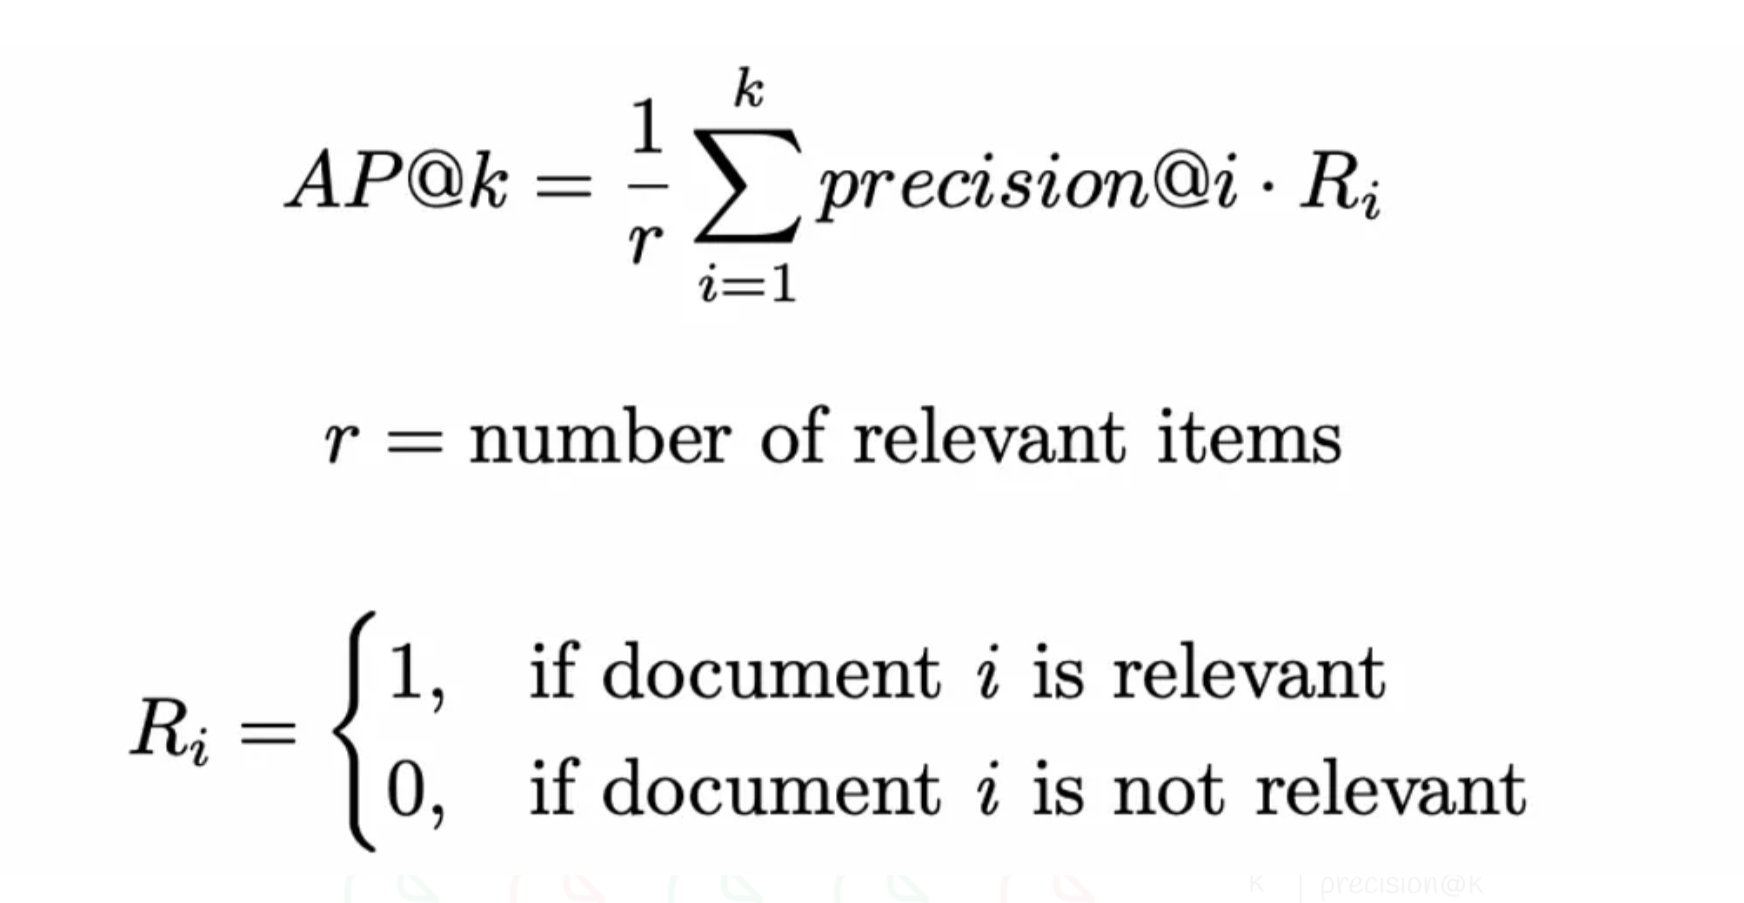
\includegraphics[width=9cm]{figure/42-ap.png}
		\citebutton{Source: towardsdatascience}{https://towardsdatascience.com/comprehensive-guide-to-ranking-evaluation-metrics-7d10382c1025}
\end{figure}

\vfill

\end{vbframe}

% ------------------------------------------------------------------------------

\begin{vbframe}{task-specific evaluation: ranking (3)}

\vfill

\textbf{Example MAP:}

\begin{figure}
    \centering
    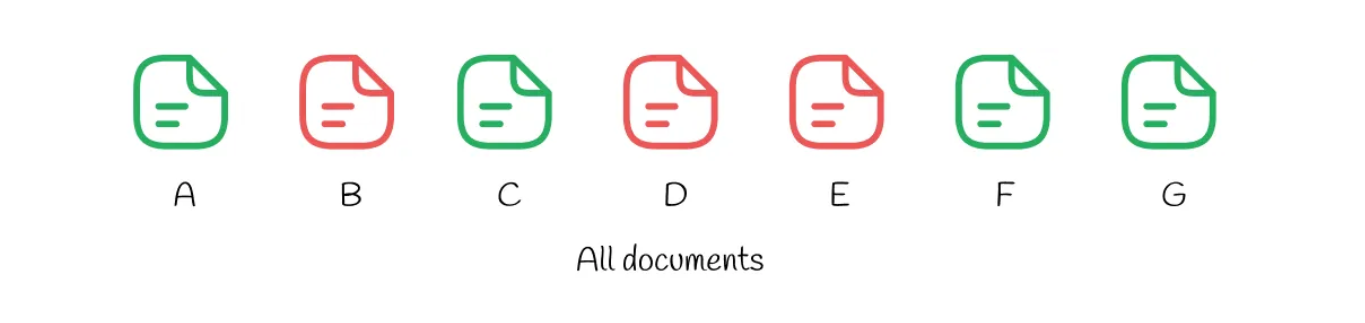
\includegraphics[width=9cm]{figure/42-ap-ex1.png}
		\citebutton{Source: towardsdatascience}{https://towardsdatascience.com/comprehensive-guide-to-ranking-evaluation-metrics-7d10382c1025}
\end{figure}

\vfill

\end{vbframe}

% ------------------------------------------------------------------------------

\begin{vbframe}{task-specific evaluation: ranking (4)}

\vfill

\textbf{Example MAP:}

\begin{figure}
    \centering
    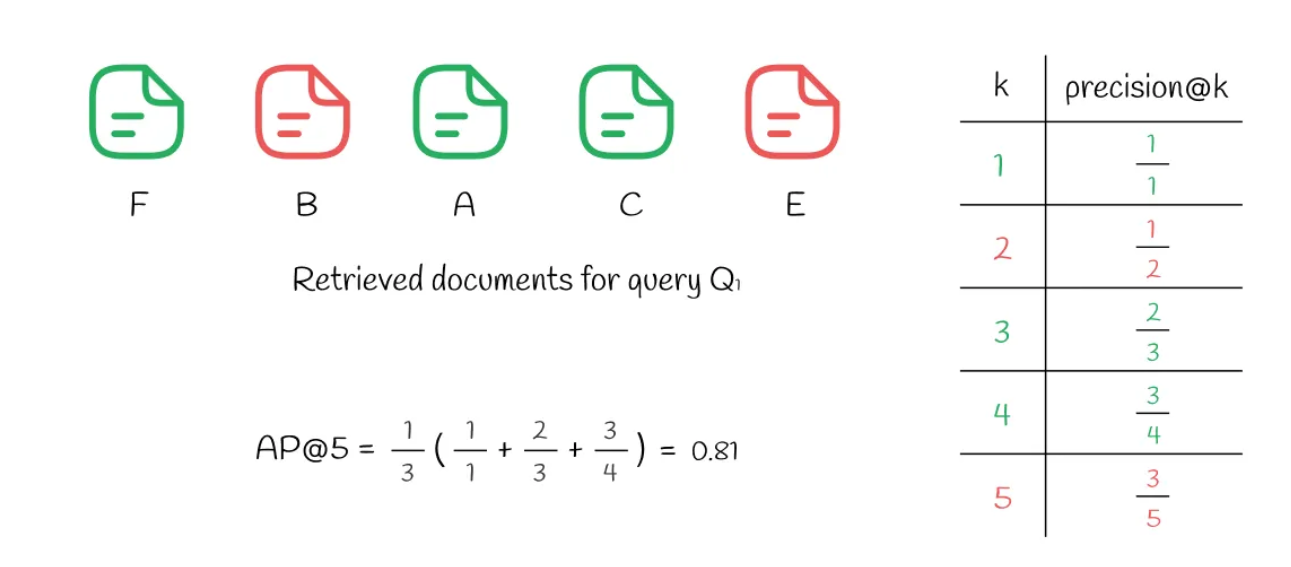
\includegraphics[width=9cm]{figure/42-ap-ex2.png}
		\citebutton{Source: towardsdatascience}{https://towardsdatascience.com/comprehensive-guide-to-ranking-evaluation-metrics-7d10382c1025}
\end{figure}

\vfill

\end{vbframe}

% ------------------------------------------------------------------------------

\begin{vbframe}{task-specific evaluation: ranking (5)}

\vfill

\textbf{Example MAP:}

\begin{figure}
    \centering
    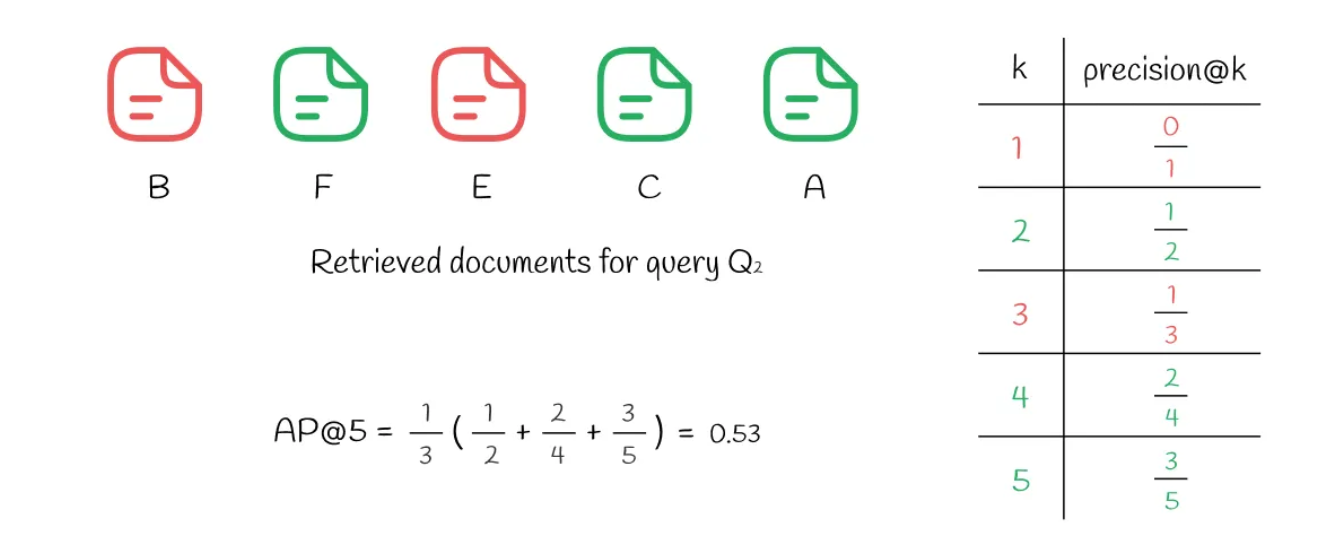
\includegraphics[width=9cm]{figure/42-ap-ex3.png}
		\citebutton{Source: towardsdatascience}{https://towardsdatascience.com/comprehensive-guide-to-ranking-evaluation-metrics-7d10382c1025}
\end{figure}

\vfill

\end{vbframe}

% ------------------------------------------------------------------------------

\begin{vbframe}{task-specific evaluation: ranking (6)}

\vfill

\textbf{MAP:}
%https://towardsdatascience.com/comprehensive-guide-to-ranking-evaluation-metrics-7d10382c1025

$$MAP = \dfrac{1}{|Q|} \sum_{q \in Q} Ap_q@k,\; with\; Q = \text{set of queries}$$

\begin{figure}
    \centering
    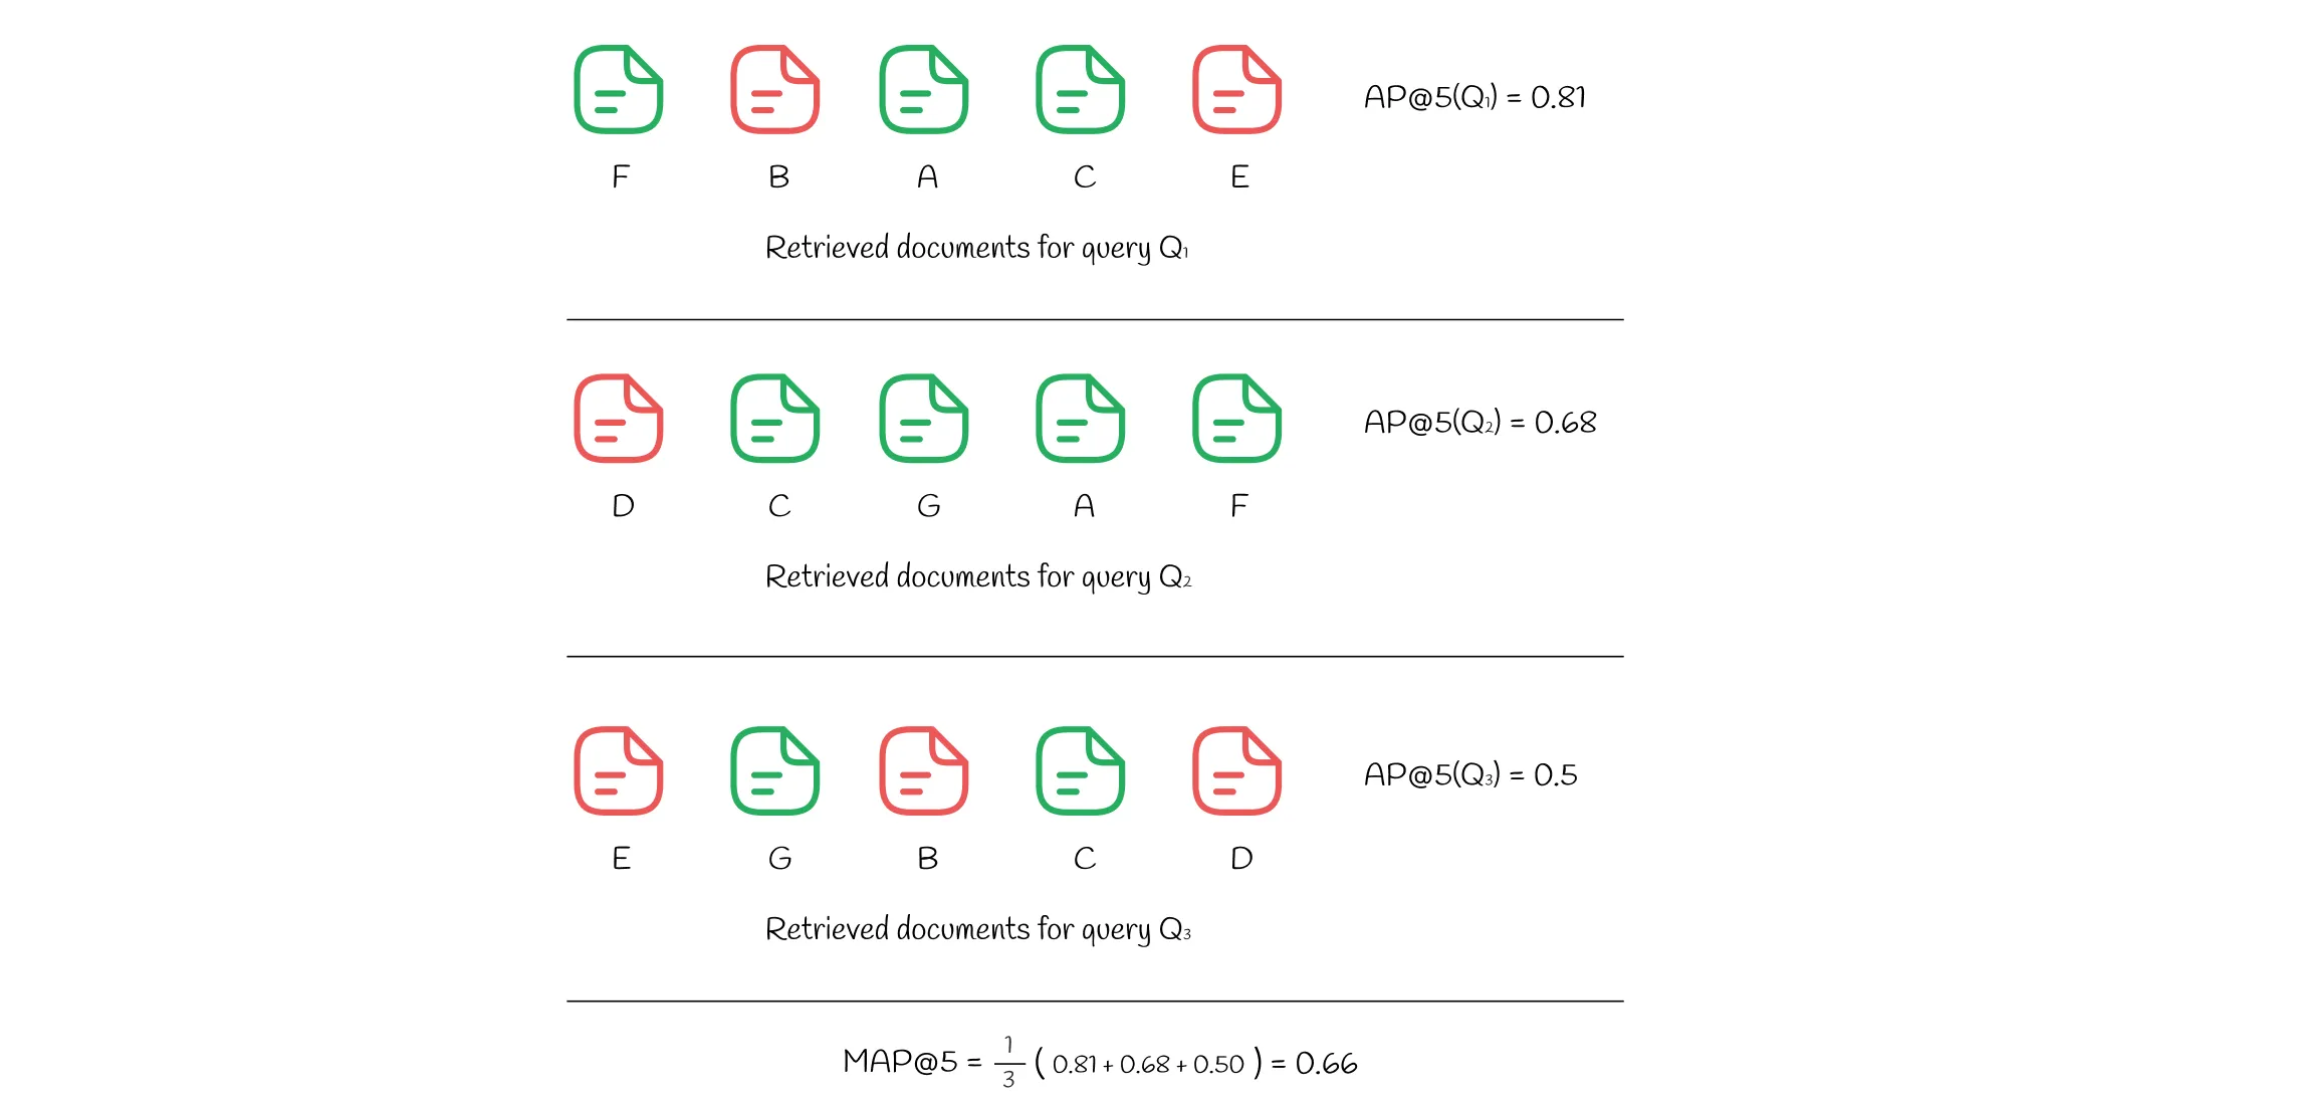
\includegraphics[width=9cm]{figure/42-ap-ex4.png}
		\citebutton{Source: towardsdatascience}{https://towardsdatascience.com/comprehensive-guide-to-ranking-evaluation-metrics-7d10382c1025}
\end{figure}

\vfill

\end{vbframe}

% ------------------------------------------------------------------------------

\begin{vbframe}{task-specific evaluation: ranking (7)}

\vfill

\textbf{MRR:}
%https://towardsdatascience.com/comprehensive-guide-to-ranking-evaluation-metrics-7d10382c1025

$$RR = \dfrac{1}{\text{rank of first relevant item}}$$
$$MRR = \dfrac{1}{|Q|} \sum_{q \in Q} RR_q,\; with\; Q = \text{set of queries}$$

\vfill

\end{vbframe}

% ------------------------------------------------------------------------------

\begin{frame}{ARLMs}

\vspace{-1cm}

	\begin{figure}
		\centering
		
\includegraphics[width=10cm,page=13]{figure/arlm.pdf}
	\end{figure}
	
\begin{itemize}
	\item \ques How can we measure ``performance`` on this task? 
\end{itemize}

\vfill

\end{frame}

% ------------------------------------------------------------------------------

\begin{frame}{arlm perplexity (1)}

\vfill

\begin{itemize}
	\item Natural choice for evaluating generated text
	\item Well-defined for ARLMs; trickier for MLMs
	\item Intuitively: \textit{Amount of the model's surprisal when confronted with a sequence} (higher value means higher ``surprisal``)
	\item More technically: Measure of uncertainty of a probabilistic model
	\item Example: Perplexity of a fair $k$-sided die (uniform distribution) is $k$
\end{itemize}

\vfill

\end{frame}

% ------------------------------------------------------------------------------

\begin{frame}{arlm perplexity (2)}

\vfill
\begin{itemize}
	\item Autoregressive factorization of the sequence:
\end{itemize}

\begin{figure}
    \centering
    \animategraphics[loop,autoplay,height=1.5cm]{2}{figure/ppl_full/frame_}{0}{11}
		\citebutton{Source: huggingface}{https://huggingface.co/docs/transformers/perplexity}
\end{figure}

\begin{itemize}
	\item Log-probability of i-th token given context: $\log(p_\theta(w_i|w_{<i}))$
	\item[] more ``certain`` model $\to$ higher log-probability
	\item Aggregate$^1$ over the whole sequence:
				$$PPL = \exp\left(\frac{1}{t} \sum_{i=1}^t \log(p_\theta(w_i|w_{<i}))\right)$$
\end{itemize}

\vfill

\footnotesize{$^1$The choice of the log’s base is basically arbitrary.}

\end{frame}

% ------------------------------------------------------------------------------

\begin{frame}{arlm perplexity (3)}

\vfill

\begin{itemize}
	\item \textit{Lower bound} is \textbf{1}, i.e. the model predicts \textit{every} token correctly (with a certainty of 100\%)
	\item \ques Is this really desirable?
	\item \textit{Upper bound} is $|V|$, i.e. the model only provides a random guess for every token with a probability of $\frac{1}{|V|}$
	\item Selection of state-of-the-art perplexities:
			\begin{itemize}
				\item \textbf{1B Word Benchmark} \citebutton{Chelba et al., 2013}{https://arxiv.org/abs/1312.3005} ($|V| = 800k$)\\
				PPL = 21,8 \citebutton{Dai et al., 2019}{https://aclanthology.org/P19-1285/}
				\item \textbf{WikiText-103} \citebutton{Merity et al., 2016}{https://arxiv.org/abs/1609.07843} ($|V|$ = 270k)\\
				PPL = 10,8 \citebutton{Shoeybi et al., 2019}{https://arxiv.org/abs/1909.08053}
				\item \textbf{Penn Treebank} \citebutton{Marcus et al., 1994}{https://aclanthology.org/H94-1020/} ($|V| = 10k$)\\
				PPL = 20,5 \citebutton{Brown et al., 2020}{https://proceedings.neurips.cc/paper_files/paper/2020/file/1457c0d6bfcb4967418bfb8ac142f64a-Paper.pdf}
			\end{itemize}
\end{itemize}

\vfill

\end{frame}

% ------------------------------------------------------------------------------

\begin{frame}{arlm perplexity (4)}

\vfill

\begin{itemize}
	\item \textit{Problem:} Fixed context size of models (e.g. 1024 for GPT-2) 
\end{itemize}

\begin{figure}
    \centering
    \animategraphics[loop,autoplay,height=1.5cm]{2}{figure/ppl_sliding/frame_}{18}{23}
		\citebutton{Source: huggingface}{https://huggingface.co/docs/transformers/perplexity}
\end{figure}

\begin{itemize}
	\item \textit{Possible solution:} Sliding window strategy
	\item Close approximation to ``true`` autoregressive decomposition
	\item \textit{Drawback:} Computationally expensive (individual forward pass for each token)
\end{itemize}

\vfill

\end{frame}

% ------------------------------------------------------------------------------

\begin{frame}{arlm perplexity (5)}

\vfill

\ques\\ Is a language model with lower perplexity always a ``better`` model?

\vspace{.5cm}

\textbf{Some (Dis)Advantages of perplexity:}

\begin{itemize}
	\item \textbf{Pro:} Straight-forward applicable
	\item \textbf{Pro:} Does not depend on ``external`` labels
	\item \textbf{Con:} Not clear what value can be considered ``good``
	\item \textbf{Con:} Corpus-/language-specific measure
\end{itemize}

\vfill

\end{frame}

% ------------------------------------------------------------------------------

\begin{vbframe}{evaluating generated text (1)}

\vfill

\begin{itemize}
	\item \ques How else can we evaluate the quality of generated text?
	\item[]
	\item \textit{Use cases:} 
			\begin{itemize}
				\item Machine translation
				\item Question answering (extractive or abstractive)
				\item Dialogue generation
				\item Text summarization
				\item Image Captioning
				\item Code generation
			\end{itemize}
\end{itemize}

\vfill

\end{vbframe}

% ------------------------------------------------------------------------------

\begin{vbframe}{evaluating generated text (2)}

\vfill

\textbf{Machine Translation}

\begin{itemize}
	\item Metrics based on N-gram-overlap
			\begin{itemize}
				\item BLEU (cf. Chap. 3.1) \citebutton{Papineni et al., 2002}{https://aclanthology.org/P02-1040/}
				\item ROUGE \citebutton{Lin, 2004}{https://aclanthology.org/W04-1013/}
				\item METEOR \citebutton{Banerjee and Lavie, 2005}{https://aclanthology.org/W05-0909/}
			\end{itemize}
	\item Metrics based pre-trained (neural) models
			\begin{itemize}
				\item BertScore \citebutton{Zhang et al., 2019}{https://arxiv.org/abs/1904.09675}
				\item BLEURT \citebutton{Sellam et al., 2020}{https://aclanthology.org/2020.acl-main.704/}
				\item COMET \citebutton{Rei et al., 2020}{https://aclanthology.org/2020.emnlp-main.213/}
			\end{itemize}
\end{itemize}

\vfill

\end{vbframe}

% ------------------------------------------------------------------------------

\begin{vbframe}{evaluating generated text (3)}

\vfill

\begin{itemize}
	\item BLEU, ROUGE, METEOR:
			\begin{itemize}
				\item "Bilingual evaluation understudy", originally for machine translation
				\item Measures overlap of words, and longer word sequences of different sizes
				\item BLEU: unreliable per-example, but correlates with human judgments on an aggregate level \citebutton{Reiter, 2018}{https://aclanthology.org/J18-3002/}
			\end{itemize}
\end{itemize}

\vfill

\end{vbframe}

% ------------------------------------------------------------------------------

\begin{vbframe}{evaluating generated text (3)}

\vfill

\begin{itemize}
	\item BERTScore
			\begin{itemize}
				\item Based on pre-trained BERT model
				\item Also able to consider contextual similarities
				\item Correlates better with human judgements
			\end{itemize}
	\item BLEURT
			\begin{itemize}
				\item Better per-example quality estimation by fine-tuning on examples with judgements
				\item But: potential bias if tested systems are very different than training examples
			\end{itemize}
\end{itemize}

\vfill

\end{vbframe}

% ------------------------------------------------------------------------------

\begin{vbframe}{evaluating generated text (4)}

\vfill

\textbf{Question Answering / Summarization / Dialogues}

\begin{itemize}
	\item Aspects to consider
			\begin{itemize}
				\item Factual correctness
				\item Fluency
				\item Stylistic aspects
				\item Engagement
				\item ...
			\end{itemize}
	\item Human evaluation?! (cf. next slide)
\end{itemize}

\vfill

\end{vbframe}

% ------------------------------------------------------------------------------

\begin{vbframe}{human evaluatoin}

\vfill

\textbf{Pros}

\begin{itemize}
	\item Possible where simply using metrics fails (esp. generated texts)
	\item Probably gold standard (given trained human evaluator)
	\item \textit{Strong} learning signal for models (cf. RLHF, chapter 9)
	\item ...
\end{itemize}

\vspace{.3cm}

\textbf{Pros}

\begin{itemize}
	\item Manual, tedious work
  \item Costs and working conditions
	\item Subjectiveness
	\item Ambiguity
	\item ...
\end{itemize}

\vfill

\end{vbframe}

% ------------------------------------------------------------------------------

\endlecture
\end{document}